
\documentclass[12pt,a4paper]{report}
\usepackage[a4paper,left=1.15in,right=0.9in,top=0.9in,bottom=0.85in]{geometry}
\usepackage{mathptmx}
\usepackage{graphicx}
\usepackage{setspace}
\usepackage{fancyhdr}
\usepackage{titlesec}
\usepackage{tocloft}
\usepackage{array}
\usepackage{booktabs}
\usepackage{longtable}
\usepackage{caption}
\usepackage{enumitem}
\usepackage[hidelinks]{hyperref}
\usepackage{ragged2e}

\graphicspath{{figures/}}
\setstretch{1.0}
\setlength{\parindent}{0pt}
\setlength{\parskip}{3pt}
\justifying
\renewcommand{\contentsname}{TABLE OF CONTENTS}
\renewcommand{\listfigurename}{LIST OF FIGURES}
\renewcommand{\listtablename}{LIST OF TABLES}
\renewcommand{\cftchapfont}{\normalfont}
\renewcommand{\cftchappagefont}{\normalfont}
\renewcommand{\cftdotsep}{1}
\captionsetup{font=bf,labelfont=bf,justification=centering}
\renewcommand{\thefigure}{\thechapter.\arabic{figure}}
\renewcommand{\thetable}{\thechapter.\arabic{table}}
\renewcommand{\figurename}{Fig.}
\renewcommand{\cftfigpresnum}{Fig. }
\setlength{\cftfignumwidth}{0.75in}
\renewcommand{\cfttabpresnum}{Table }
\setlength{\cfttabnumwidth}{0.9in}

\titleformat{\chapter}
  {\normalfont\bfseries\centering\fontsize{16}{19}\selectfont}
  {CHAPTER \thechapter}{0.5em}{\MakeUppercase}
\titlespacing*{\chapter}{0pt}{6pt}{6pt}
\titleformat{name=\chapter,numberless}
  {\normalfont\bfseries\centering\fontsize{16}{19}\selectfont}
  {}{0pt}{\MakeUppercase}
\titleformat{\section}
  {\normalfont\bfseries\fontsize{14}{17}\selectfont}
  {\thesection}{3em}{\MakeUppercase}
\titlespacing*{\section}{0pt}{5pt}{2pt}
\titleformat{\subsection}
  {\normalfont\bfseries\fontsize{12}{15}\selectfont}
  {\thesubsection}{3em}{}
\titlespacing*{\subsection}{0pt}{6pt}{2pt}

\newcommand{\studentid}{23AIML010}
\newcommand{\chapterheader}{CHAPTER HEADING}
\fancyhf{}
\fancyhead[L]{\fontsize{10}{12}\selectfont\studentid}
\fancyhead[R]{\fontsize{10}{12}\selectfont\chapterheader}
\fancyfoot[L]{\fontsize{10}{12}\selectfont DEPSTAR}
\fancyfoot[C]{\fontsize{10}{12}\selectfont\thepage}
\fancyfoot[R]{\fontsize{10}{12}\selectfont Department of Computer Engineering}
\renewcommand{\headrulewidth}{0pt}
\renewcommand{\footrulewidth}{0pt}

\newcommand{\frontchapter}[1]{\chapter*{#1}\addcontentsline{toc}{chapter}{#1}\markboth{#1}{#1}}

\begin{document}
\pagestyle{empty}
\pagenumbering{gobble}
\begin{titlepage}
\thispagestyle{empty}
\begin{singlespace}
\centering

\includegraphics[width=3.4in]{charusat_logo.png}\par
\vspace{0.18in}
{\bfseries\fontsize{16}{19}\selectfont A SUMMER INTERNSHIP REPORT\par}
\vspace{0.12in}
{\bfseries\fontsize{14}{17}\selectfont ON\par}
\vspace{0.12in}
{\bfseries\fontsize{16}{19}\selectfont ECOROUTE ENGINE\par}
\vspace{0.14in}
{\bfseries\fontsize{13}{16}\selectfont Geospatial Fleet Routing and Dispatch Optimization Platform\par}
\vspace{0.16in}
Submitted in partial fulfilment of the requirements for the Summer Internship\par
\vspace{0.13in}
{\bfseries Bachelor of Technology\par}
in\par
{\bfseries Computer Engineering\par}
\vspace{0.18in}
{\bfseries Submitted by\par}
{\bfseries\fontsize{14}{17}\selectfont OM CHIRAGBHAI CHOKSI\par}
{\bfseries 23AIML010\par}
\vspace{0.15in}
{\bfseries Internship Organization\par}
Logicwind\par
{\bfseries Internship Duration\par}
Six months ongoing, started from 1 June 2026\par
Current report status: first month completed, five months remaining\par
\vspace{0.12in}
{\bfseries Under the Guidance of\par}
[Internal Guide Name]\par
[Designation]\par
\vspace{0.22in}
{\bfseries\fontsize{14}{17}\selectfont Department of Computer Engineering\par}
{\bfseries\fontsize{13}{16}\selectfont Devang Patel Institute of Advance Technology and Research (DEPSTAR)\par}
Charotar University of Science and Technology, Changa\par
\vspace{0.08in}
{\bfseries July 2026\par}
\end{singlespace}
\end{titlepage}

\chapter*{College Certificate}
This is to certify that the Summer Internship report entitled ``EcoRoute Engine'' has been carried out by OM CHIRAGBHAI CHOKSI, bearing Student ID 23AIML010, under my supervision and guidance during the academic year 2026. The internship at Logicwind is planned for six months. This interim report records the work, technical study and learning completed after the first month.

\vspace{1.0in}
\begin{center}
\begin{tabular}{p{0.45\textwidth}p{0.45\textwidth}}
\centering\rule{2.3in}{0.4pt} & \centering\arraybackslash\rule{2.3in}{0.4pt}\\
\centering Internal Guide & \centering\arraybackslash Head of Department
\end{tabular}
\end{center}
\vfill

\noindent\textbf{Company / Organization Certificate:} Official certificate from Logicwind to be inserted when available.

\vfill

\noindent\textbf{Declaration by the Candidate:} I hereby declare that this internship report submitted to DEPSTAR, CHARUSAT, is a record of bonafide internship learning carried out at Logicwind. This report represents the first completed month of a six-month ongoing internship.

\vspace{0.15in}
\begin{flushright}
\rule{2.2in}{0.4pt}\\
OM CHIRAGBHAI CHOKSI\\
23AIML010
\end{flushright}
\clearpage

\pagestyle{fancy}
\pagenumbering{roman}
\setcounter{page}{1}
\renewcommand{\chapterheader}{PRELIMINARY PAGES}
\frontchapter{Acknowledgement}
I express my sincere gratitude to Logicwind for giving me the opportunity to work in a professional backend development environment. During the first month of internship, I learned how software tasks are planned, assigned, reviewed and improved through structured communication, Git workflow and ClickUp-based tracking.

I am thankful to my company mentors and senior team members for their guidance in backend architecture, API design, security practices and project implementation. I also thank my internal guide [Internal Guide Name], the Department of Computer Engineering, DEPSTAR and CHARUSAT for academic support and encouragement.
\clearpage

\frontchapter{Abstract}
This report presents the first-month work and learning completed during an ongoing six-month summer internship at Logicwind. The internship started on 1 June 2026. At the time of this report, one month has been completed and five months are still remaining. The main focus of the first month was backend engineering, REST API design, secure backend development, database design, documentation and professional workflow.

The project studied in detail is EcoRoute Engine, a backend infrastructure platform for geospatial fleet routing, pickup dispatch and circular economy logistics. It is designed for organization-scoped operations including business location management, pickup request lifecycle, vehicle capacity management, driver assignment, dispatch execution, route generation, OSRM-based routing, dashboard analytics, audit logging and notification delivery. The backend uses Node.js, Express.js, TypeScript, PostgreSQL with PostGIS, Zod validation, JWT authentication, RBAC middleware, Docker Compose and a layered routes-controllers-services-repositories architecture. The inspected codebase includes approximately seventeen route modules, sixteen controllers, sixteen services, sixteen repositories, eight SQL migration files, and ten test files covering health, auth, businesses, pickups, vehicles, dispatch, routes, dashboard and audit domains.
\clearpage

\tableofcontents
\clearpage
% \listoffigures
% \clearpage
% \listoftables
% \clearpage

\frontchapter{Description of Company / Organization}
Logicwind is a software development organization where I received exposure to practical backend development and professional project workflow. The internship environment helped me understand how development tasks move from requirement discussion to implementation, review, testing and documentation. ClickUp was used as a task planning and tracking tool, while Git-based workflow helped maintain change history and collaboration discipline. The team follows structured development practices including task assignment through ClickUp, feature branch creation, pull request reviews, code quality checks, testing and deployment planning. Communication with mentors and senior developers was conducted through regular sync meetings and status updates.

\pagenumbering{arabic}
\setcounter{page}{1}
\renewcommand{\chapterheader}{CHAPTER 1}
\chapter{Introduction and Internship Overview}

\section{Internship Context}
The internship at Logicwind is a six-month ongoing internship that started on 1 June 2026. This report is prepared after the first completed month, so it is an interim record rather than a final completion report. The first month helped me understand backend development from a professional viewpoint: requirement study, API planning, secure implementation, database design, code review and documentation.

The internship environment uses ClickUp for task tracking, Git and GitHub for version control, and regular code reviews for quality assurance. I was assigned to study, explore and document the EcoRoute Engine backend platform. The work involved reading existing source code, understanding API structure, examining database schemas, studying security middleware, understanding transaction patterns and preparing technical documentation.

\section{Project Overview}
EcoRoute Engine is a backend infrastructure platform designed to optimize commercial waste collection, recycling logistics and circular economy transportation operations. The platform leverages geospatial intelligence, route optimization algorithms and real-world road network analysis to automatically assign pickup requests to available vehicles, generate optimized collection routes and maximize fleet utilization while respecting operational constraints such as vehicle capacity, service areas and travel distance.

The system uses PostgreSQL with PostGIS for spatial analysis and Open Source Routing Machine (OSRM) for high-performance route computation based on OpenStreetMap data. It provides dispatch automation, route planning, fleet monitoring and operational analytics through a scalable backend architecture. Key domain modules include organizations, users, businesses, pickup locations, waste categories, vehicles, drivers, pickup requests, dispatch assignment, route generation, route stops, vehicle location tracking, notifications, dashboard metrics and audit logging.

\section{Objectives and Scope}
The major objectives of the first month were to strengthen backend fundamentals, understand REST API structure, study JWT authentication and RBAC, learn PostgreSQL and PostGIS schema design, understand OSRM-based routing concepts, compare REST with GraphQL, practise Git workflow and document technical work in academic format.

The scope of work includes requirement analysis of the existing codebase, study of layered backend architecture, examination of security controls, understanding of transactional dispatch operations, review of database migration design, analysis of OSRM integration patterns, and preparation of structured documentation. The work does not include frontend implementation, production deployment, load testing or performance benchmarking.

\begin{figure}[h!]
\centering
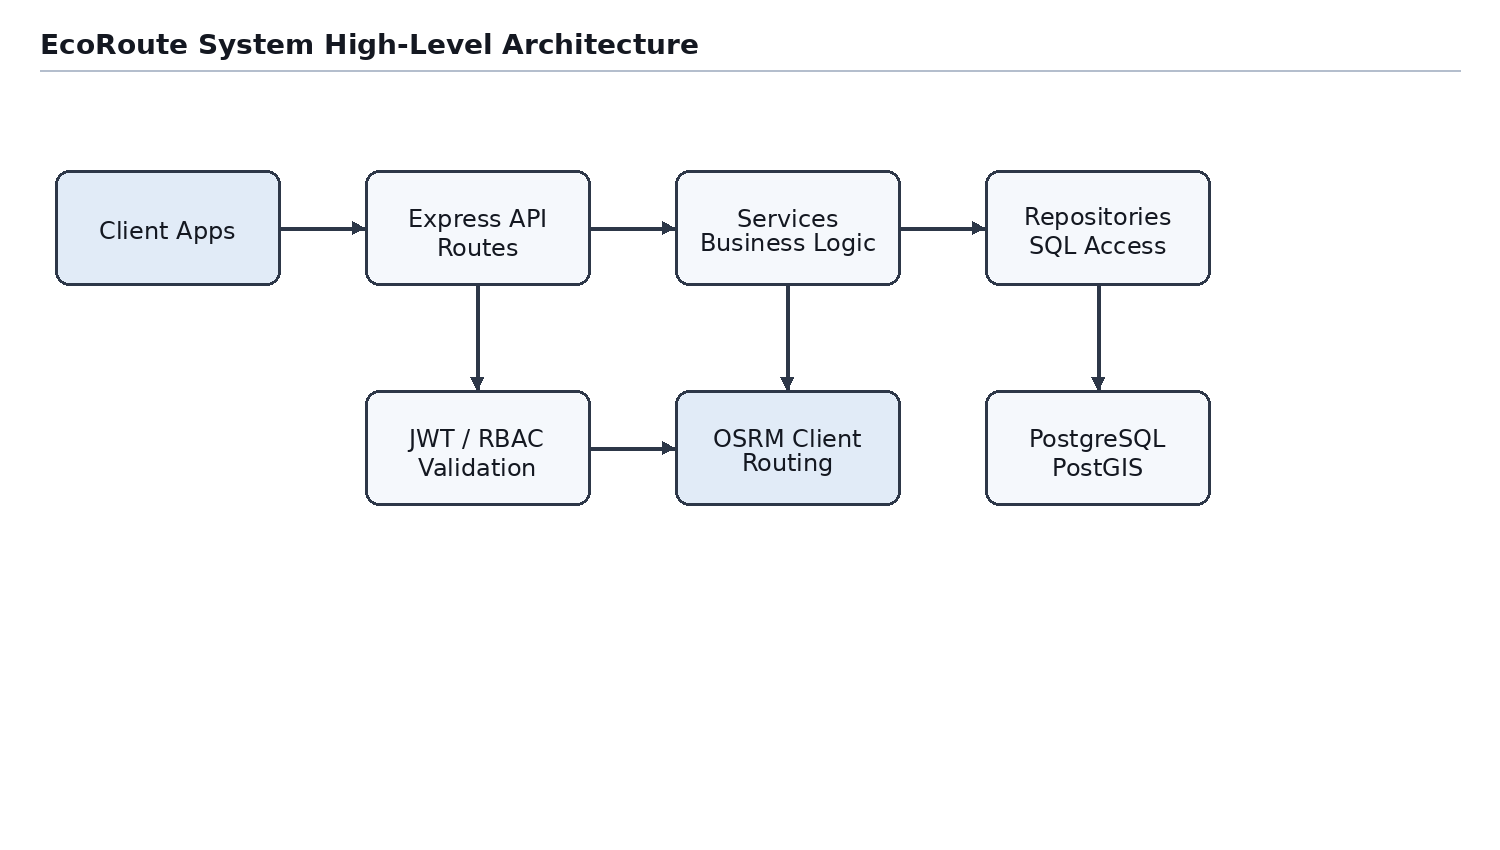
\includegraphics[width=0.85\textwidth]{architecture_high_level.png}
\caption{High-Level Architecture of EcoRoute Engine}
\end{figure}

\section{Report Organization}
The report is organized into five chapters. Chapter 1 introduces the internship context and project overview. Chapter 2 describes the technology stack, tools and validation patterns used in the backend. Chapter 3 presents the system architecture, layered design, database schema and API structure. Chapter 4 discusses implementation details of critical modules, testing methodology and documentation. Chapter 5 presents learning outcomes, future scope and conclusion, followed by references.
\clearpage

\renewcommand{\chapterheader}{CHAPTER 2}
\chapter{Technology Stack and Development Environment}

\section{Backend Runtime and Framework}
EcoRoute Engine is built on Node.js with TypeScript using the Express.js framework. TypeScript provides static type checking, interface definitions and improved code maintainability across the large module set. Express handles HTTP routing, middleware composition and request-response processing. The type definitions for Express request objects are augmented to include authenticated user payloads, enabling type-safe access to user identity, organization scope and role information inside controllers and services.

The backend package configuration lists dependencies including bcryptjs for password hashing, jsonwebtoken for JWT creation and verification, pg for PostgreSQL database connectivity, zod for request validation, helmet for HTTP security headers, cors for cross-origin support, express-rate-limit for rate limiting, swagger-ui-express for API documentation, and resend for email delivery. Dev dependencies include TypeScript compiler, ts-node for development execution, nodemon for auto-restart, Jest and Supertest for testing.

\section{Database and Spatial Extensions}
PostgreSQL serves as the primary database with the PostGIS extension enabled for geospatial data storage and querying. The businesses table includes a geography column of type GEOGRAPHY(POINT, 4326) with a GIST index for spatial lookup performance. Spatial queries such as finding nearby pickup requests or computing distances between business locations can be executed directly in the database layer using PostGIS functions.

Database access is managed through the pg connection pool configured with a maximum of ten connections, connection timeout of five seconds and idle timeout of thirty seconds. A helper function withTransaction accepts a callback that runs inside a database transaction with automatic commit and rollback. This pattern is used extensively in the dispatch and route generation modules to ensure atomic state transitions.

\begin{table}[h!]
\centering
\caption{Technology Stack Summary}
\begin{tabular}{|p{1.4in}|p{4.0in}|}
\hline
\textbf{Area} & \textbf{Technologies and Practices}\\\hline
Runtime & Node.js, TypeScript, Express.js, ts-node, nodemon\\\hline
Database & PostgreSQL 16, PostGIS 3.4, pg connection pool, parameterized SQL\\\hline
Validation & Zod schemas with safeParse, UUID format checks, string constraints\\\hline
Authentication & JWT access tokens, JWT refresh tokens, configurable expiry\\\hline
Authorization & RBAC middleware for admin, dispatcher, driver roles\\\hline
API Documentation & OpenAPI 3.0.3 specification, Swagger UI express middleware\\\hline
Security & Helmet, CORS with explicit origin, bcrypt, rate limiting on auth endpoints\\\hline
Routing Engine & OSRM client with nearest, table, trip endpoints, offline stub mode\\\hline
Testing & Jest test runner, Supertest HTTP assertions, module-level mocking\\\hline
Containerization & Docker, Docker Compose, multi-service orchestration\\\hline
Task Tracking & ClickUp for task assignment, priority, status tracking\\\hline
Version Control & Git, GitHub, feature branch workflow, pull request reviews\\\hline
\end{tabular}
\end{table}

\section{Validation and Error Handling}
Request validation is performed using Zod schemas defined in the schemas directory. Each write endpoint has a corresponding schema that validates the shape, type and format of the request body. For example, the dispatch assign schema requires a valid UUID for vehicleId and a non-empty array of UUID strings for pickupIds. The auth register schema enforces minimum password length of eight characters, trims whitespace and converts email to lowercase. Schemas export inferred TypeScript types so that services receive fully typed input objects.

Error handling follows a custom hierarchy built on the AppError base class. Subclasses include ValidationError for 400 responses, UnauthorizedError for 401, ForbiddenError for 403, NotFoundError for 404 and ConflictError for 409. A global error handler middleware catches all errors, maps status codes to string identifiers and returns a consistent JSON response structure. Stack traces are included only in non-production environments. Server errors are logged at error level while client errors are logged at warn level, both as structured JSON with request path and method information.

\section{Configuration and Environment Management}
Application configuration is loaded from environment variables using dotenv. The configuration module defines a typed AppConfig interface covering server port, database credentials, JWT secrets and expiry times, OSRM base URL and timeout, offline mode flags, logging preferences, rate limit parameters and email service settings. Required variables throw descriptive errors at startup if missing. The config object and its nested objects are frozen to prevent accidental mutation at runtime.

Feature flags are organized under an offline configuration group. These flags control whether OSRM calls return live data or stubs, whether external APIs are enabled, whether notifications, email, SMS and queue processing are active. This design allows the system to run fully offline without external dependencies during development and testing.
\clearpage

\renewcommand{\chapterheader}{CHAPTER 3}
\chapter{System Design and Architecture}

\section{Layered Backend Architecture}
The backend is organized into five distinct layers. Express route files define HTTP method, path and middleware chains. Controllers extract validated input from the request, call services and send standardized responses. Validation schemas defined in Zod enforce request body structure at the API boundary. Services contain domain business logic including validation rules, state transitions and integration orchestration. Repositories encapsulate SQL query execution and return typed row objects.

This separation makes each layer independently testable. Controllers can be tested with mocked services using Supertest. Services can be tested with mocked repositories. Repositories can be tested with an isolated test database. The architecture follows established backend patterns and avoids mixing HTTP concerns with business logic or database access.

\begin{figure}[h!]
\centering
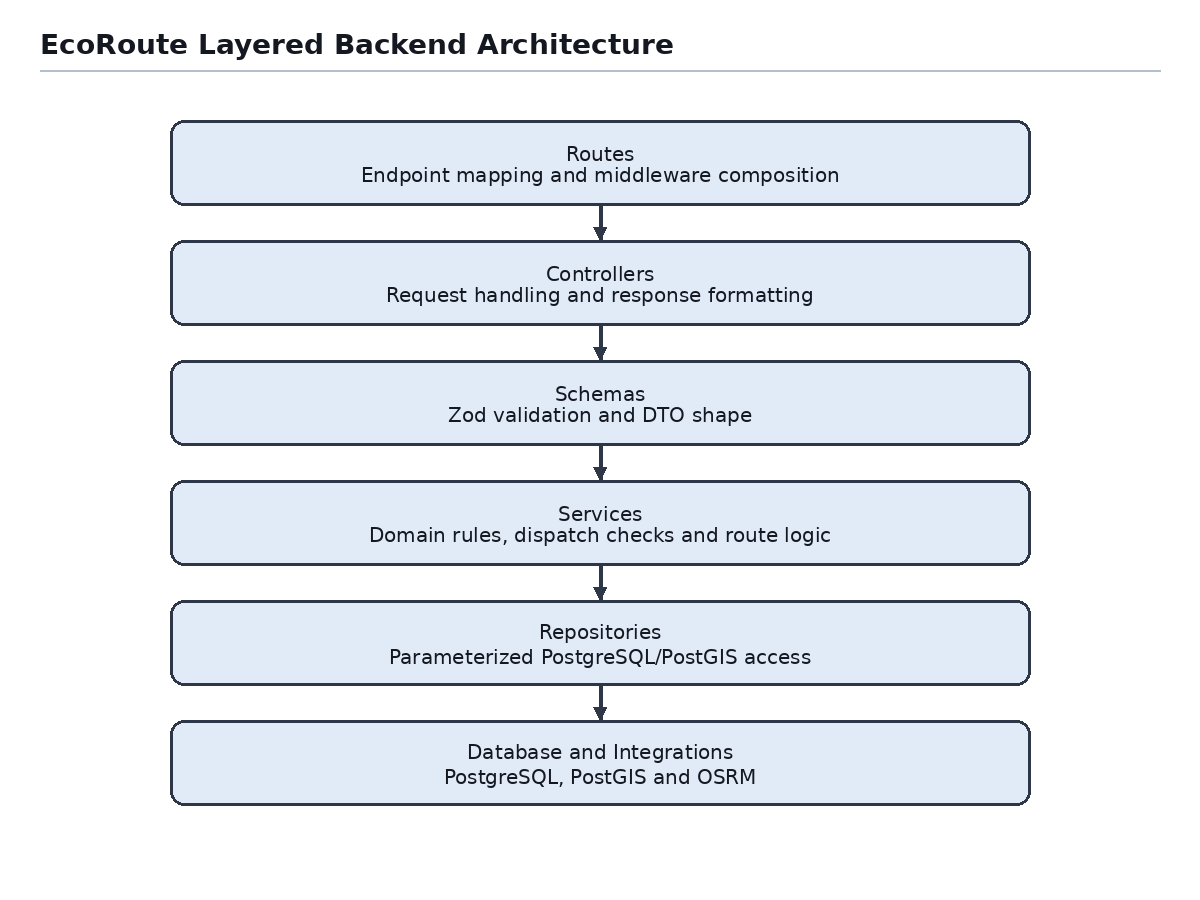
\includegraphics[width=0.82\textwidth]{architecture_layered.png}
\caption{Layered Backend Architecture of EcoRoute Engine}
\end{figure}

\section{Database Schema and Migration Design}
The database schema is built incrementally through eight SQL migration files executed in order. The migrations create tables for organizations, users, businesses, vehicles, pickup requests, routes, audit logs and password reset OTPs. Each migration is wrapped in a transaction block and includes index creation for foreign keys and filtered query paths.

The businesses table includes a PostGIS geography column with a GIST spatial index for location-based queries. Check constraints enforce latitude range between -90 and 90, longitude range between -180 and 180, positive vehicle capacity and valid current load range. The vehicles table includes a unique constraint on the combination of organization ID and plate number to prevent duplicate registration within an organization.

The routes table includes a partial unique index that prevents more than one active route per vehicle at any given time. Status columns across all tables use CHECK constraints to restrict allowed values. Foreign key relationships enforce referential integrity with appropriate delete behaviours including CASCADE, RESTRICT and SET NULL depending on the entity relationship.

\section{API Design and Routing Structure}
The API follows RESTful conventions with a versioned prefix of /api/v1. Route files are organized by domain and registered in the central app module. A root index endpoint at /api/v1 returns a complete listing of all available endpoints organized by domain category, serving as a developer reference.

The authentication module provides register, login, refresh, forgot-password and reset-password endpoints. Protected domain routes include organizations, users, businesses, pickup locations, waste categories, vehicles, drivers, pickups, dispatch, routes, route stops, vehicle locations, notifications, dashboard and audit logs. Each domain typically supports list, create, get-by-id and update operations with appropriate access controls.

\begin{table}[h!]
\centering
\caption{API Domain Modules and Endpoint Count}
\begin{tabular}{|p{1.8in}|p{1.5in}|p{2.0in}|}
\hline
\textbf{Domain Module} & \textbf{Endpoints} & \textbf{Authentication}\\\hline
Authentication & 5 endpoints & Public with rate limiting\\\hline
Organizations & 4 endpoints & Authenticated\\\hline
Users & 5 endpoints & Authenticated, admin role\\\hline
Businesses & 4 endpoints & Authenticated\\\hline
Pickup Locations & 5 endpoints & Authenticated\\\hline
Waste Categories & 4 endpoints & Authenticated\\\hline
Vehicles & 5 endpoints & Authenticated\\\hline
Drivers & 6 endpoints & Authenticated\\\hline
Pickups & 7 endpoints & Authenticated\\\hline
Dispatch & 3 endpoints & Authenticated, dispatcher or admin\\\hline
Routes & 6 endpoints & Authenticated\\\hline
Routing & 4 endpoints & Authenticated\\\hline
Dashboard & 7 endpoints & Authenticated\\\hline
Notifications & 5 endpoints & Authenticated\\\hline
Audit Logs & 1 endpoint & Authenticated, admin\\\hline
\end{tabular}
\end{table}

\section{Security Architecture}
Authentication is implemented through JWT access tokens and refresh tokens. The access token has a configurable short expiry while the refresh token has a longer expiry. The authenticate middleware extracts the Bearer token from the Authorization header, verifies it using the JWT secret and attaches the decoded payload to the request object. The payload includes user ID, organization ID, role and email.

Authorization is enforced through the requireRole middleware which accepts a variable list of allowed roles. If the authenticated user role is not in the allowed list, a ForbiddenError is raised. This middleware is applied at the route level so that sensitive operations such as dispatch assignment, audit log access and user role management are restricted to admin or dispatcher roles.

Additional security controls include Helmet for HTTP header protection, CORS configured with the frontend origin, bcrypt password hashing with configurable salt rounds, rate limiting on authentication endpoints with a limit of ten requests per window, and consistent error messages that do not reveal whether an email exists in the database during login or password reset.
\clearpage

\renewcommand{\chapterheader}{CHAPTER 4}
\chapter{Implementation Details and Testing}

\section{Authentication and User Management}
The authentication module implements registration, login, token refresh, password reset via OTP and password change. Registration creates an organization and an admin user in a single database transaction. Both organization email and user email are checked for uniqueness before creation. The password is hashed using bcrypt before storage. On success, the response includes user details, organization details and both access and refresh tokens.

Login validates credentials by fetching the user by email, comparing the password hash using bcrypt and generating tokens. The same error message is returned for both invalid email and incorrect password to prevent user enumeration. Token refresh verifies the refresh token using a separate secret, looks up the user and generates a new token pair.

Password reset uses a six-digit OTP hashed with bcrypt and stored with an expiry time. The OTP is validated against the hash, checked for expiry and limited to five attempts before requiring a new OTP. On successful verification, the password is updated and the OTP is marked as used. Welcome email and password reset email are sent through the mail service using the Resend API when email is enabled.

\section{Dispatch Module}
The dispatch module is the most critical business component because it handles the transition of pickups from pending to assigned state and vehicles from available to dispatched state. It must protect against duplicate assignment, capacity overflow and inconsistent state under concurrent dispatcher activity.

The assign dispatch endpoint accepts a vehicle ID and an array of pickup IDs. It executes inside a database transaction with the following sequence. First, the vehicle row is locked using SELECT FOR UPDATE to prevent concurrent modification. If the vehicle status is not available, a conflict error is raised. Second, all requested pickup rows are locked using SELECT FOR UPDATE. If the number of returned rows does not match the requested IDs, a not-found error is raised.

Third, each pickup is checked for pending status. If any pickup is already assigned or in progress, a conflict error is raised listing the problematic pickup IDs. Fourth, the total weight of all pickups is calculated and compared against the available capacity of the vehicle. If the total weight exceeds the available capacity, a conflict error is raised with the specific capacity values.

Fifth, the vehicle status is updated to dispatched and the current load is incremented. Sixth, the pickups are updated to assigned status with the vehicle ID set. The update query includes a WHERE clause that checks status equals pending and assigned vehicle ID is null, preventing race conditions where another transaction may have modified the pickups between the lock and the update. If the number of updated pickups does not match the requested count, a conflict error is raised indicating concurrent assignment.

Finally, an audit log entry is written recording the actor, action type, entity ID and metadata including pickup IDs and count. If any step in this sequence fails, the entire transaction is rolled back, ensuring no partial state changes persist.

\begin{figure}[h!]
\centering
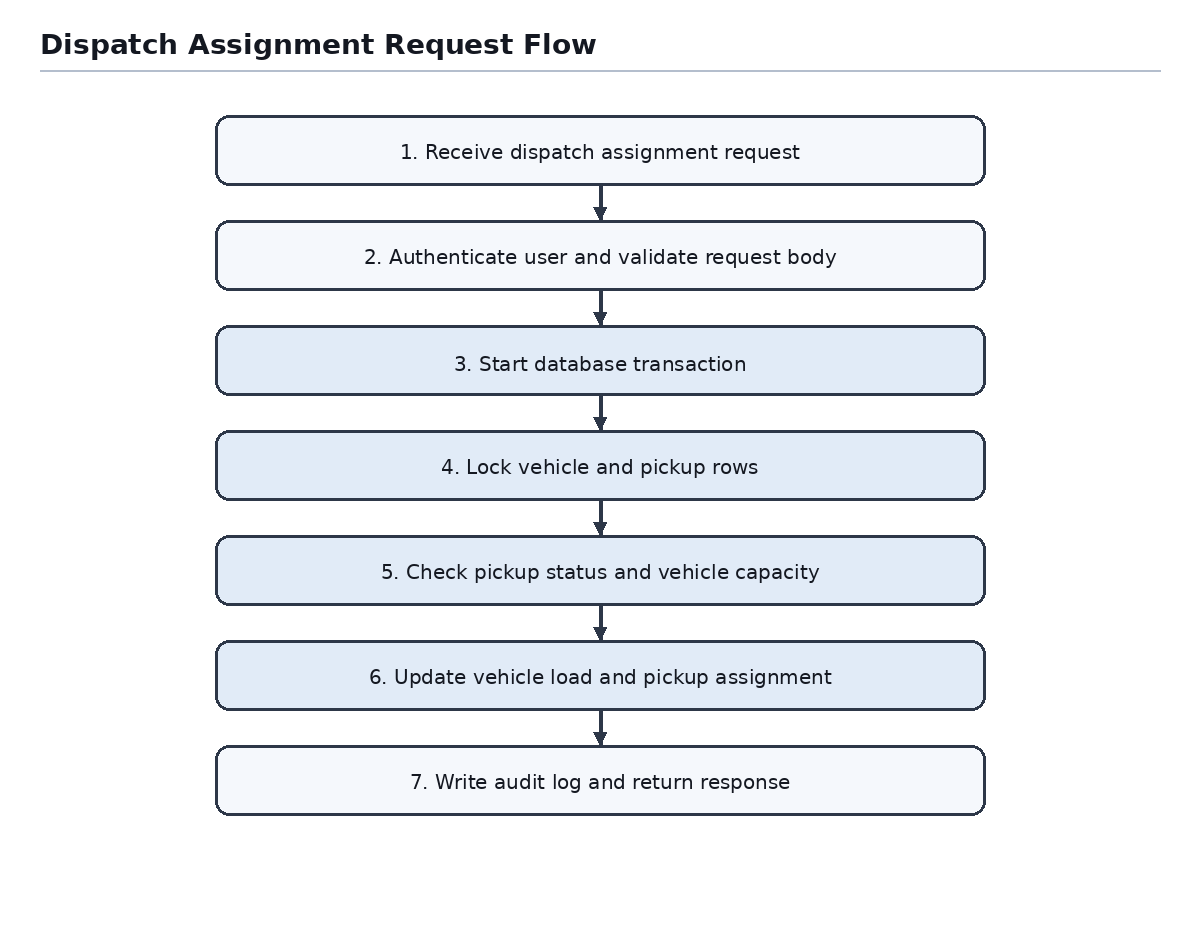
\includegraphics[width=0.88\textwidth]{dispatch_request_flow.png}
\caption{Dispatch Assignment Request Flow with Transaction Boundaries}
\end{figure}

The auto-assign endpoint provides an alternative workflow that automatically distributes unassigned pending pickups across available vehicles. It iterates through available vehicles, assigns pickups up to the configured maximum per vehicle and respects optional weight limits per vehicle. Each vehicle assignment is executed in its own transaction to maximize throughput while maintaining per-assignment atomicity.

\section{Route Generation and Routing Integration}
Route generation creates an optimized collection route for a dispatched vehicle. It executes inside a transaction to maintain consistency with the dispatch state. The vehicle is locked and verified to be in dispatched status. An active route check prevents duplicate route creation using the partial unique index. Assigned pickups are fetched along with their geographic coordinates through a spatial join between the pickup requests table and the businesses table using PostGIS geometry extraction functions.

The pickup coordinates are sent to the OSRM trip endpoint which computes an optimized stop order, total distance, total duration and route geometry. The OSRM client is designed with offline mode support. When OFFLINE\_MODE is enabled, the client returns stub results with zero distances and empty geometries. This allows development and testing without a running OSRM instance. The trip endpoint uses the driving profile with roundtrip set to false, source set to first and destination set to last.

On successful OSRM response, a route record is created with distance, duration, geometry, waypoints and raw OSRM data stored as JSONB. The associated pickups are updated to in-progress status with the route ID set. If the OSRM call fails or returns an unexpected response, the error propagates up the call stack and the transaction is rolled back, preventing incomplete route data from being persisted.

Route completion transitions the route to completed status, resets the vehicle to available with zero current load and marks all associated pickups as completed. These three operations execute atomically inside a single transaction with row-level locking on the route record.

\section{Testing Methodology}
The backend includes ten test files covering all major modules. Tests are written using Jest as the test runner and Supertest for HTTP-level assertions. External dependencies including the database pool, repository modules and bcryptjs are mocked at the module level using jest.mock. This ensures tests run without requiring a live database or external service.

The test setup file configures environment variables with test-specific values including a test JWT secret, test database URL and offline mode enabled. The withTransaction helper is mocked to execute the provided callback immediately with a mock client object, allowing tests to verify transaction behaviour without a database connection.

\begin{table}[h!]
\centering
\caption{Test Coverage Summary}
\begin{tabular}{|p{1.5in}|p{4.0in}|}
\hline
\textbf{Test Module} & \textbf{Verification Focus}\\\hline
Health & Database connectivity check, OSRM status reporting, overall degraded status\\\hline
Authentication & Registration success, duplicate email conflict, login validation, token refresh, rate limiting, no password hash exposure\\\hline
Businesses & CRUD operations, organization scoping, validation error handling\\\hline
Pickups & Creation, status transitions, cancellation, nearby search\\\hline
Vehicles & Create, update status, assign driver, organization isolation\\\hline
Dispatch & Successful assignment, empty pickup IDs, non-UUID input, missing token, vehicle not found, vehicle not available, pickup not found, pickup already assigned, concurrent assignment race, capacity exceeded, exact capacity boundary\\\hline
Routes & Route generation, OSRM integration, completion flow, state validation\\\hline
Dashboard & Summary metrics, vehicle workloads, pickup statistics, fleet utilization\\\hline
Audit & Audit log creation, retrieval, organization-scoped filtering\\\hline
\end{tabular}
\end{table}

The dispatch test suite is the most comprehensive, covering twelve distinct scenarios including success path, validation failures, authentication errors, not-found conditions, status conflicts, capacity boundary tests and concurrent assignment detection. The concurrent assignment test verifies that when the update query returns zero rows because pickups were assigned by another transaction, the service raises a conflict error with a descriptive message.

\section{Docker and Deployment Configuration}
Docker Compose defines three services. The database service uses the postgis/postgres image with health check using pg\_isready. The backend service builds from the local Dockerfile, exposes port 3000 and depends on the database health check. Environment variables are passed from the host environment with sensible defaults for development.

A migrate service runs under the tools profile and executes all SQL migration files against the database in order. On first startup, migrations also execute automatically through the docker-entrypoint-initdb.d volume mount on the database container. The OSRM service is documented in a commented block, requiring preprocessed OpenStreetMap data in the OSM PBF format processed through OSRM extraction, partition and customization commands.

The Dockerfile uses a multi-stage build with a dependency installation stage and a runtime stage. The application runs as a non-root node user for security. Health check endpoints are configured for both the database and backend services to support container orchestration.

\clearpage

\renewcommand{\chapterheader}{CHAPTER 5}
\chapter{Learning Outcomes, Future Scope and Conclusion}

\section{Learning Outcomes}
The first month of internship at Logicwind provided practical exposure to production-oriented backend development. Through the study of EcoRoute Engine, I learned how a real-world backend is organized into routes, controllers, validation schemas, services and repositories. I understood why each layer exists and how separation of concerns improves maintainability, testability and code clarity.

I learned how JWT authentication works in practice including token generation, verification, expiry management and the distinction between access tokens and refresh tokens. I understood how RBAC middleware restricts endpoint access based on user roles and why organization-level scoping is important for multi-tenant applications.

The dispatch module taught me about transactional consistency, row-level locking and concurrent access protection. I learned that checking conditions and persisting changes inside the same transaction with appropriate lock levels prevents race conditions that would otherwise cause duplicate assignments or capacity violations.

I gained practical knowledge of PostgreSQL and PostGIS including geography column types, GIST spatial indexes, check constraints, partial unique indexes and parameterized query patterns. I learned how SQL migrations are structured, ordered and executed to evolve the database schema safely.

On the security side, I understood the importance of input validation at the API boundary, consistent error messages that do not leak information, rate limiting on sensitive endpoints, password hashing with bcrypt, HTTP security headers and environment-based secret configuration.

I also learned professional habits such as reading existing code before making changes, writing clear documentation, tracking tasks through ClickUp, using Git feature branches, communicating progress with mentors and preparing structured reports. The internship environment helped me understand how development teams collaborate through code reviews, issue tracking and regular communication.

\section{Future Scope}
The remaining five months of the internship provide opportunities for deeper involvement in backend development. Future work can include implementing additional API features, writing integration tests with a test database, improving error handling and logging, adding request validation for edge cases and contributing to frontend integration using the Next.js application in the repository.

Advanced topics for further study include queue-based asynchronous job processing for route computation, WebSocket-based real-time vehicle tracking, caching strategies for frequently accessed data, performance profiling and optimization, and production deployment practices including CI/CD pipeline configuration, monitoring and alerting.

The EcoRoute Engine project has potential for extension including richer dashboard visualizations, notification delivery through multiple channels, driver mobile application support, integration with external mapping services, enhanced route optimization algorithms and machine learning-based demand prediction for pickup scheduling.

\section{Conclusion}
The first month of the Logicwind internship gave me practical exposure to production-oriented backend development through the study of EcoRoute Engine. I examined a realistic backend codebase involving REST APIs, TypeScript, authentication and authorization, PostgreSQL and PostGIS spatial databases, OSRM routing integration, Docker containerization, OpenAPI documentation and automated testing.

I learned how layered architecture, transactional dispatch, row-level locking and capacity validation work together to create a reliable dispatch system. I understood the importance of security controls including JWT authentication, RBAC middleware, input validation, rate limiting and secure password handling. I gained experience reading production code, understanding API structures, examining database schemas and preparing technical documentation.

This experience has strengthened my backend engineering foundation and will support deeper learning and more independent contribution during the remaining five months of the internship. The structured approach to system design, security, testing and documentation observed in this project provides a reference for future academic and professional work.
\clearpage

\renewcommand{\chapterheader}{REFERENCES}
\chapter*{References}
\addcontentsline{toc}{chapter}{References}
\begin{enumerate}[label={[\arabic*]},leftmargin=0.3in,itemsep=2pt]
\item EcoRoute Engine repository documentation, \texttt{README.md}, inspected from the local project repository.
\item EcoRoute backend documentation, \texttt{backend/README.md}, inspected from the local project repository.
\item EcoRoute product requirements, \texttt{docs/project.md}, inspected from the local project repository.
\item EcoRoute backend source code, \texttt{backend/src}, inspected from the local project repository.
\item EcoRoute SQL migrations, \texttt{backend/db/migrations}, inspected from the local project repository.
\item Docker Compose configuration, \texttt{docker-compose.yml}, inspected from the local project repository.
\item Frontend Next.js application files, \texttt{frontend}, inspected from the local project repository.
\item Express.js Documentation, \url{https://expressjs.com/}
\item Node.js Documentation, \url{https://nodejs.org/docs/latest/api/}
\item TypeScript Documentation, \url{https://www.typescriptlang.org/docs/}
\item PostgreSQL Documentation, \url{https://www.postgresql.org/docs/}
\item PostGIS Documentation, \url{https://postgis.net/documentation/}
\item Open Source Routing Machine Documentation, \url{https://project-osrm.org/docs/}
\item OpenAPI Specification, \url{https://spec.openapis.org/oas/latest.html}
\item Swagger UI Documentation, \url{https://swagger.io/tools/swagger-ui/}
\item JSON Web Token Introduction, \url{https://jwt.io/introduction}
\item Bcrypt password hashing, \url{https://www.npmjs.com/package/bcryptjs}
\item Zod validation library, \url{https://zod.dev/}
\item Jest testing framework, \url{https://jestjs.io/docs/getting-started}
\item Supertest HTTP assertions, \url{https://www.npmjs.com/package/supertest}
\item Docker Documentation, \url{https://docs.docker.com/}
\item Apollo GraphQL Documentation, \url{https://www.apollographql.com/docs/}
\item GraphQL Documentation, \url{https://graphql.org/learn/}
\item Mermaid Diagram Syntax Documentation, \url{https://mermaid.js.org/syntax/flowchart.html}
\item CHARUSAT reference report format, used for logo and academic front-matter reference.
\end{enumerate}

\end{document}
